\documentclass{article}
\usepackage{amsmath, amssymb}
\usepackage{tikz}
\usepackage{graphicx}
\usepackage[margin=1in, landscape]{geometry}
\usetikzlibrary{shapes, arrows, positioning, calc}

\begin{document}

% =========================
% Token Generation + Loss (Forward) - FINAL Z label update
% =========================
\noindent
\resizebox{\linewidth}{!}{%
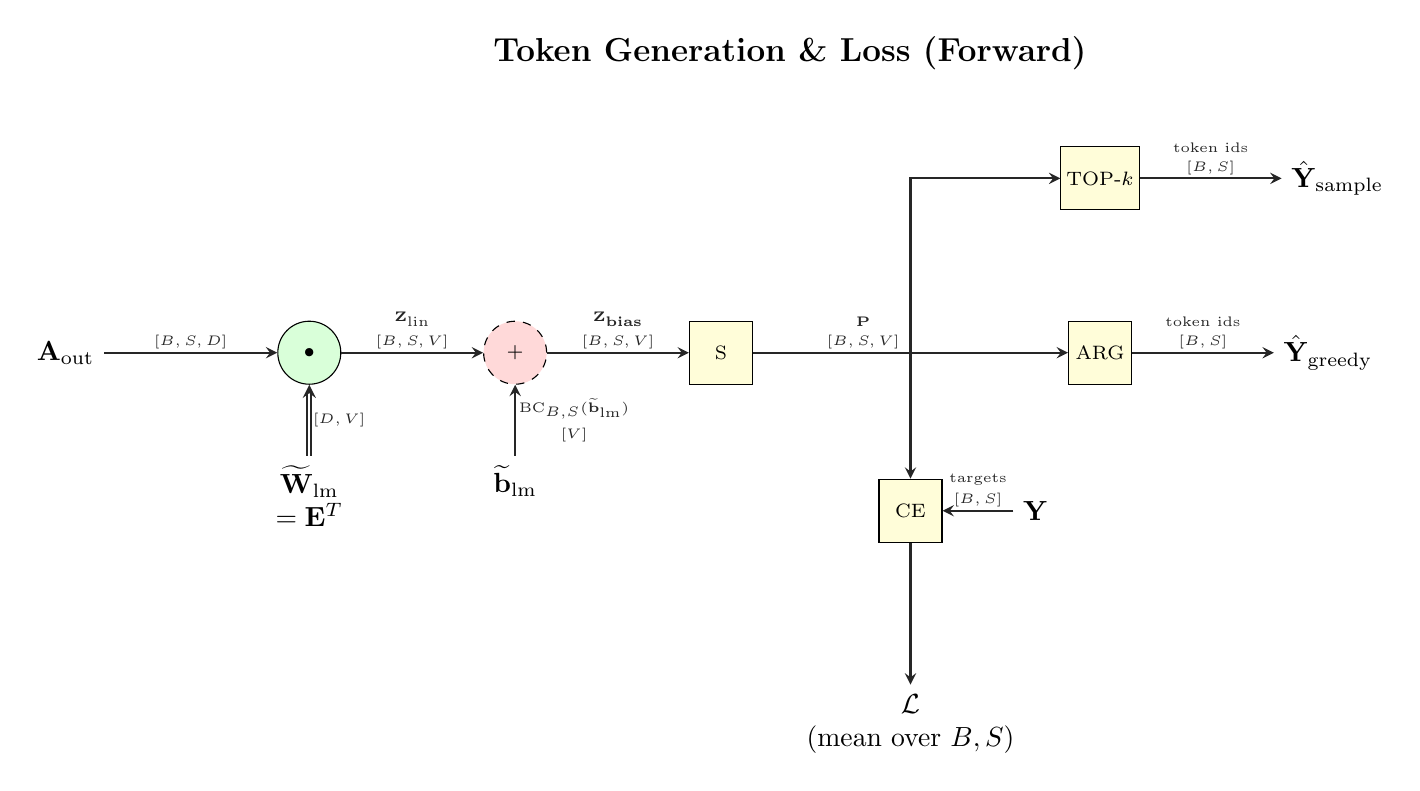
\begin{tikzpicture}[
  >=stealth,
  auxnode/.style={draw, rectangle, fill=yellow!15, minimum height=8mm, minimum width=8mm, inner sep=2pt, font=\scriptsize, align=center},
  mulnode/.style={draw, circle, fill=green!15, minimum size=8mm, font=\scriptsize, align=center},
  addnode/.style={draw, circle, dashed, fill=red!15, minimum size=8mm, font=\scriptsize, align=center},
  sumnode/.style={draw, circle, fill=red!25, minimum size=6mm, font=\tiny, align=center},
  flow/.style={->, thick, black!85},
  flow2/.style={double, ->, thick, black!85},
  dimlabel/.style={font=\tiny, inner sep=1pt, align=center}
]

% From Transformer output
\node            (H)     at (0,-2) {$\mathbf{A}_{\text{out}}$};

% LM head
\node[mulnode]   (LMmul) [right=2.2cm of H] {$\bullet$};
\node            (Wlm)   [align=center, below=0.9cm of LMmul] {$\widetilde{\mathbf{W}}_{\text{lm}}$\\$=\mathbf{E}^{T}$};
\node[addnode]   (AddB)  [right=1.8cm of LMmul] {+};
\node            (blm)   [below=0.9cm of AddB] {$\widetilde{\mathbf{b}}_{\text{lm}}$};

% Softmax → Prob
\node[auxnode]   (SM)    [right=1.8cm of AddB] {S};

\node[auxnode] (ARG)  [right=4.0cm of SM] {ARG};
% Midpoint of SM→P edge (for CE tap)
\coordinate (MidSP) at ($(SM)!0.5!(ARG)$);

% CE node placed below the SM→P edge
\node[auxnode]   (CE)    [below=1.6cm of MidSP] {CE};
\node            (Y)     [right=0.9cm of CE] {$\mathbf{Y}$};
\node            (Loss)  [align=center, below=1.8cm of CE] {$\mathcal{L}$\\ (mean over $B,S$)};
% Flows
\draw[flow]  (H) -- (LMmul) node[dimlabel, midway, above]{\shortstack{$[B,S,D]$}};
\draw[flow2] (Wlm) -- (LMmul) node[dimlabel, midway, right]{\shortstack{$[D,V]$}};
\draw[flow]  (LMmul) -- (AddB) node[dimlabel, midway, above]{\shortstack{$\mathbf{Z}_{\text{lin}}$\\$[B,S,V]$}}; % Linear output
\draw[flow]  (blm) -- (AddB)   node[dimlabel, midway, right]{\shortstack{$\text{BC}_{B,S}(\widetilde{\mathbf{b}}_{\text{lm}})$\\$[V]$}};
\draw[flow]  (AddB) -- (SM)    node[dimlabel, midway, above]{\shortstack{\textbf{Z\textsubscript{bias}}\\ $[B,S,V]$}}; % FINAL LOGITS Z_bias

% Tap the SM→P edge downward into CE
\draw[flow]  (MidSP) -- (CE);
% Targets into CE
\draw[flow]  (Y) -- (CE)  node[dimlabel, midway, above]{\shortstack{targets\\$[B,S]$}};
% Loss goes WEST (left) from CE
\draw[flow]  (CE) -- (Loss);


\node           (YhatG) [right=1.8cm of ARG] {$\hat{\mathbf{Y}}_{\text{greedy}}$};

\draw[flow] (SM) -- (ARG)
  node[dimlabel, pos=0.35, above]{\shortstack{$\mathbf{P}$\\$[B,S,V]$}};
\draw[flow] (ARG) -- (YhatG)
  node[dimlabel, midway, above]{\shortstack{token ids\\$[B,S]$}};

% Optional: top-k (or nucleus) sampling path
\node[auxnode] (TopK) [above=1.4cm of ARG] {TOP-$k$};
\node           (YhatS) [right=1.8cm of TopK] {$\hat{\mathbf{Y}}_{\text{sample}}$};

\draw[flow] (MidSP) |- (TopK);
\draw[flow] (TopK) -- (YhatS)
  node[dimlabel, midway, above]{\shortstack{token ids\\$[B,S]$}};

\node[font=\large\bfseries] at (9.2,1.8) {Token Generation \& Loss (Forward)};


\end{tikzpicture}%
}


\vspace{0.9cm}

% =========================
% Token Generation + Loss (Backward) - FINAL Z label update
% =========================
\noindent
\resizebox{0.8\linewidth}{!}{%
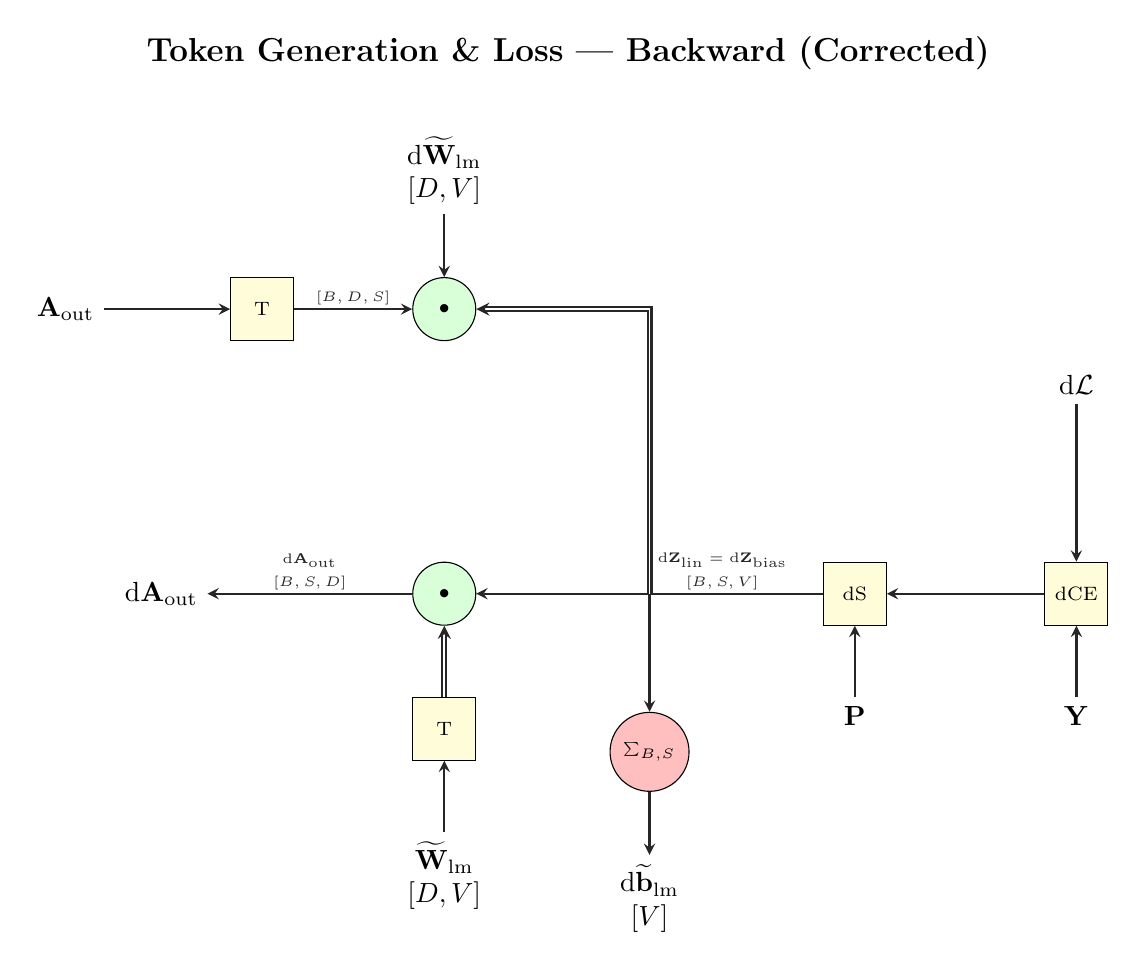
\begin{tikzpicture}[
  >=stealth,
  auxnode/.style={draw, rectangle, fill=yellow!15, minimum height=8mm, minimum width=8mm, inner sep=2pt, font=\scriptsize, align=center},
  mulnode/.style={draw, circle, fill=green!15, minimum size=8mm, font=\scriptsize, align=center},
  addnode/.style={draw, circle, dashed, fill=red!15, minimum size=8mm, font=\scriptsize, align=center},
  sumnode/.style={draw, circle, fill=red!25, minimum size=8mm, font=\tiny, align=center},
  flow/.style={<-, thick, black!85},
  flow2/.style={double, <-, thick, black!85},
  fwd/.style={->, thick, black!85},
  gradflow/.style={->, thick, black!85}, % For gradients flowing to weights/bias
  dimlabel/.style={font=\tiny, inner sep=1pt, align=center}
]

% Start from dL
\node           (dL)    at (18,0) {$\text{d}\mathcal{L}$};
\node[auxnode]  (dCE)   [below=2.0cm of dL] {dCE};
\node           (Y)     [below=0.9cm of dCE] {$\mathbf{Y}$};

% Softmax backward
\node[auxnode]  (dS)   [left=2.0cm of dCE] {dS};
\node           (P)     [below=0.9cm of dS] {$\mathbf{P}$};


% Logits (Linear Projection) backprop node
\node[mulnode]  (backMul) [left=4.4cm of dS] {$\bullet$};
\node[auxnode]  (T_Wlm)   [below=0.9cm of backMul] {T};
\node           (Wlm)     [align=center, below=0.9cm of T_Wlm] {$\widetilde{\mathbf{W}}_{\text{lm}}$\\$[D,V]$};

\coordinate (B_split) at ($(backMul)!0.5!(dS)$);

% SUM node for Bias gradient
\node[sumnode]  (SumB) [below=1.5cm of B_split] {$\sum_{B,S}$};
\node           (db)   [align=center, below=0.8cm of SumB] {$\text{d}\widetilde{\mathbf{b}}_{\text{lm}}$\\$[V]$};


% dW calc
\node[mulnode]  (dWmul) [above=2.8cm of backMul] {$\bullet$};
\node[auxnode]  (TAout) [left=1.5cm of dWmul] {T};
\node           (Aout)  [left=1.6cm of TAout] {$\mathbf{A}_{\text{out}}$};
\node           (dW)    [align=center, above=0.8cm of dWmul] {$\text{d}\widetilde{\mathbf{W}}_{\text{lm}}$\\$[D,V]$};

% Back to Transformer
\node           (dH)    [left=2.6cm of backMul] {$\text{d}\mathbf{A}_{\text{out}}$};
\coordinate (MiddZ) at ($(B_split)!0.5!(dS)$);


% Flows

% 1. Loss and dS to dAddB (dZ_bias)
\draw[flow] (dCE) -- (dL);
\draw[fwd]  (Y) -- (dCE);
\draw[flow] (dS) -- (dCE);
\draw[fwd]  (P) -- (dS);

% 2. Bias Gradient Calculation
\draw[gradflow] (B_split) -- (SumB.north);
\draw[gradflow] (SumB) -- (db);

% 3. Linear Projection Backprop (dZ_bias -> dZ_lin, dH)
\draw[flow] (backMul) -- (dS) node[dimlabel, pos=0.71, above]{\shortstack{$\text{d}\mathbf{Z}_{\text{lin}}=\text{d}\mathbf{Z}_{\text{bias}}$\\$[B,S,V]$}}; % dZ_lin flows from dAddB to backMul
\draw[flow2] (backMul) -- (T_Wlm);
\draw[fwd]   (Wlm) -- (T_Wlm);
\draw[flow]  (dH) -- (backMul) node[dimlabel, midway, above]{\shortstack{$\text{d}\mathbf{A}_{\text{out}}$\\$[B,S,D]$}};


% 4. dW Calculation
\draw[gradflow] (dW) -- (dWmul);
\draw[fwd]  (Aout) -- (TAout);
\draw[fwd]  (TAout) -- (dWmul) node[dimlabel, midway, above]{\shortstack{$[B,D,S]$}};
\draw[flow2] (dWmul) -| (B_split); % dZ_bias flows to dWmul


\node[font=\large\bfseries, anchor=south]
  at ([yshift=6mm]current bounding box.north) {Token Generation \& Loss — Backward (Corrected)};
\end{tikzpicture}%
}

% =========================
% Abbreviation Tables (new page) - FINAL Z label update
% =========================
\newpage
\renewcommand{\arraystretch}{1.2}
\small

% -------- Operations (Ops) --------
\begin{center}
\textbf{Operations (Ops)}
\begin{tabular}{llll}
\hline
\textbf{Abbrev} & \textbf{Name} & \textbf{Type / Shape} & \textbf{Notes} \\
\hline
S     & Softmax                     & op            & Over vocab axis $V$; outputs probabilities $\mathbf{P}$. \\
CE    & Cross-Entropy               & op            & Usually \emph{sparse} CE consuming label indices $\mathbf{Y}$. \\
ARG   & Argmax (greedy)             & op            & $\operatorname*{argmax}_V$ to get token ids (no gradient). \\
TOP-$k$ & Top-$k$ / sampling        & op            & Optional decoding path (or nucleus sampling); no gradient. \\
T     & Transpose                   & op            & E.g., $\widetilde{\mathbf{W}}_{\text{lm}}^{T} \in \mathbb{R}^{V\times D}$. \\
$\mathrm{BC}_{B,S}(\cdot)$ & Broadcast & op       & Expand $[V] \!\to\! [B,S,V]$ for bias add. \\
dS    & Softmax backward            & op            & The output is $\mathrm{d}\mathbf{Z}_{\text{bias}} = \mathbf{P}-\text{onehot}(\mathbf{Y})$ (with CE). \\
dAddB & Addition (Bias) backward & op            & Passes $\mathrm{d}\mathbf{Z}_{\text{bias}}$ to $\mathrm{d}\mathbf{Z}_{\text{lin}}$ and $\sum_{B,S}$.\\
$\sum_{B,S}$ & Summation            & op            & Sums $\mathrm{d}\mathbf{Z}_{\text{bias}}$ over axes $B$ and $S$ to get $\mathrm{d}\widetilde{\mathbf{b}}_{\text{lm}}$.\\
\hline
\end{tabular}
\end{center}

\vspace{0.8em}

% -------- Data Tensors (Values) --------
\begin{center}
\textbf{Data Tensors (Values)}
\begin{tabular}{lllp{0.46\linewidth}}
\hline
\textbf{Symbol} & \textbf{Name} & \textbf{Shape} & \textbf{Notes} \\
\hline
$\mathbf{A}_{\text{out}}$ & Transformer output (hidden) & $[B,S,D]$ & Final hidden from the Transformer block(s). \\
$\widetilde{\mathbf{W}}_{\text{lm}}$ & LM head weight (tied) & $[D,V]$ & Typically tied to $\mathbf{E}^{T}$. \\
$\widetilde{\mathbf{b}}_{\text{lm}}$ & LM head bias           & $[V]$    & Broadcast-added over $[B,S,V]$. \\
$\mathbf{Z}_{\text{lin}}$ & Logits (linear output) & $[B,S,V]$ & $\mathbf{Z}_{\text{lin}}=\mathbf{A}_{\text{out}}\widetilde{\mathbf{W}}_{\text{lm}}$. \\
$\mathbf{Z}_{\text{bias}}$ & Logits (final/Softmax input) & $[B,S,V]$ & $\mathbf{Z}_{\text{bias}}=\mathbf{Z}_{\text{lin}}+\widetilde{\mathbf{b}}_{\text{lm}}$. \\
$\mathbf{P}$ & Probabilities                     & $[B,S,V]$ & $\mathbf{P}=\mathrm{softmax}(\mathbf{Z}_{\text{bias}})$. \\
$\mathbf{Y}$ & Target token ids                  & $[B,S]$   & Ground-truth indices (sparse labels). \\
$\mathcal{L}$ & Loss                              & scalar or $[B,S]$ & Typically mean over $B,S$. \\
$\mathrm{d}\mathcal{L}$ & Loss gradient          & scalar-grad & Starting signal for backward pass. \\
$\mathrm{d}\mathbf{Z}_{\text{bias}}$  & Final Logits gradient  & $[B,S,V]$  & From CE+Softmax: $\mathbf{P}-\text{onehot}(\mathbf{Y})$. \\
$\mathrm{d}\mathbf{Z}_{\text{lin}}$ & Linear output grad & $[B,S,V]$ & Same as $\mathrm{d}\mathbf{Z}_{\text{bias}}$ (input to $\mathbf{Z}_{\text{lin}}$ matmul). \\
$\mathrm{d}\widetilde{\mathbf{W}}_{\text{lm}}$ & LM weight grad & $[D,V]$ & $=\mathbf{A}_{\text{out}}^{T}\mathrm{d}\mathbf{Z}_{\text{lin}}$. \\
$\mathrm{d}\widetilde{\mathbf{b}}_{\text{lm}}$ & LM bias grad & $[V]$ & $=\sum_{B,S}(\mathrm{d}\mathbf{Z}_{\text{bias}})$. \\
$\mathrm{d}\mathbf{A}_{\text{out}}$ & Hidden grad & $[B,S,D]$  & $=\mathrm{d}\mathbf{Z}_{\text{lin}}\,\widetilde{\mathbf{W}}_{\text{lm}}^{T}$. \\
\hline
\multicolumn{4}{l}{\textbf{Shapes:}\ $B$=batch,\ $S$=sequence length,\ $D$=hidden dim,\ $V$=vocab size.} \\
\hline
\end{tabular}
\end{center}

\end{document}